%!TEX root = ../2015_06_16-HATS-LPC-JEC.tex

\frame{
\frametitle{What form do the corrections come in?}
\framesubtitle{Text File}
\vspace*{0.3cm}
	%\begin{textblock}{14.5}(0.0,0.7)
		\begin{center}
%			\scalebox{.9}{
				%\documentclass[dvipsnames]{standalone}
\usepackage{color}
\usepackage{tikz}
\usetikzlibrary{arrows,shapes,shapes.multipart,backgrounds,calc,decorations.text,decorations.pathreplacing,matrix,shadings}
\tikzstyle{every picture}+=[remember picture]
\tikzstyle{na} = [baseline=-.5ex]

\begin{document}

\tikzstyle{levels} = [rectangle, draw, text width=6em, text centered, rounded corners, minimum height=2em, midway, shading=radial,outer color=Gray,middle color=white,inner color=white, Gray]
\tikzstyle{arrow} = [draw, -latex']
\tikzstyle{line} = [draw, -]

\newcommand*{\mytextstyle}{\sffamily\Large\bfseries\color{black!85}}
\newcommand{\myarrowstart}[9]{%
% inner radius, middle radius, outer radius, start angle,
% end angle, tip protusion angle, options, text
  \pgfmathsetmacro{\start}{#1}
  \pgfmathsetmacro{\rin}{#2}
  \pgfmathsetmacro{\rmid}{#3}
  \pgfmathsetmacro{\rout}{#4}
  \pgfmathsetmacro{\astart}{#5}
  \pgfmathsetmacro{\aend}{#6}
  \pgfmathsetmacro{\atip}{#7}
  \fill[#8] (\start+\astart,\rin) -- (\start+\aend,\rin) -- (\start+\aend+\atip,\rmid)
        -- (\start+\aend,\rout) -- (\start+\astart,\rout) -- (\start+\astart,\rmid)
        -- cycle;
  \node[font = \sffamily, align=center,text width=\aend-\astart,anchor = west, yshift=-0.0ex] (arrowend) at (\start+\astart,\rmid) {\mytextstyle{#9}};
%  \path[font = \sffamily, decoration = {text along path, text = {|\mytextstyle|#9},
%    text align = {align = center}, raise = -0.5ex}, decorate]
%    (\start+\astart+0.4*\atip,\rmid) -- (\start+\aend+0.4*\atip,\rmid);
}
\newcommand{\myarrow}[9]{%
% inner radius, middle radius, outer radius, start angle,
% end angle, tip protusion angle, options, text
  \pgfmathsetmacro{\start}{#1}
  \pgfmathsetmacro{\rin}{#2}
  \pgfmathsetmacro{\rmid}{#3}
  \pgfmathsetmacro{\rout}{#4}
  \pgfmathsetmacro{\astart}{#5}
  \pgfmathsetmacro{\aend}{#6}
  \pgfmathsetmacro{\atip}{#7}
  \fill[#8] (\start+\astart,\rin) -- (\start+\aend,\rin) -- (\start+\aend+\atip,\rmid) 
        -- (\start+\aend,\rout) -- (\start+\astart,\rout) -- (\start+\astart+\atip,\rmid)
        -- cycle;
  \path[font = \sffamily, decoration = {text along path, text = {|\mytextstyle|#9},
    text align = {align = center}, raise = -0.5ex}, decorate]
    (\start+\astart+0.75*\atip,\rmid) -- (\start+\aend+0.75*\atip,\rmid);
}
\newcommand{\myuphalfarrow}[9]{%
% inner radius, middle radius, outer radius, start angle,
% end angle, tip protusion angle, options, text
  \pgfmathsetmacro{\start}{#1}
  \pgfmathsetmacro{\rin}{#2}
  \pgfmathsetmacro{\rmid}{#3}
  \pgfmathsetmacro{\rout}{#4}
  \pgfmathsetmacro{\astart}{#5}
  \pgfmathsetmacro{\aend}{#6}
  \pgfmathsetmacro{\atip}{#7}
  \fill[#8] (\start+\astart,\rout) -- (\start+\aend,\rout) -- (\start+\aend+\atip,\rin) 
        -- (\start+\astart+\atip,\rin) -- cycle;
  \path[font = \sffamily, decoration = {text along path, text = {|\mytextstyle|#9},
    text align = {align = center}, raise = -0.5ex}, decorate]
    (\start+\astart+0.4*\atip,\rmid) -- (\start+\aend+0.4*\atip,\rmid);
}
\newcommand{\mylowhalfarrow}[9]{%
% inner radius, middle radius, outer radius, start angle,
% end angle, tip protusion angle, options, text
  \pgfmathsetmacro{\start}{#1}
  \pgfmathsetmacro{\rin}{#2}
  \pgfmathsetmacro{\rmid}{#3}
  \pgfmathsetmacro{\rout}{#4}
  \pgfmathsetmacro{\astart}{#5}
  \pgfmathsetmacro{\aend}{#6}
  \pgfmathsetmacro{\atip}{#7}
  \fill[#8] (\start+\astart+\atip,\rin) -- (\start+\aend+\atip,\rin) -- (\start+\aend,\rout)
        -- (\start+\astart,\rout) -- cycle;
  \path[font = \sffamily, decoration = {text along path, text = {|\mytextstyle|#9},
    text align = {align = center}, raise = -0.5ex}, decorate]
    (\start+\astart+0.4*\atip,\rmid) -- (\start+\aend+0.4*\atip,\rmid);
}
\newcommand{\myarrowend}[9]{%
% inner radius, middle radius, outer radius, start angle,
% end angle, tip protusion angle, options, text
  \pgfmathsetmacro{\start}{#1}
  \pgfmathsetmacro{\rin}{#2}
  \pgfmathsetmacro{\rmid}{#3}
  \pgfmathsetmacro{\rout}{#4}
  \pgfmathsetmacro{\astart}{#5}
  \pgfmathsetmacro{\aend}{#6}
  \pgfmathsetmacro{\atip}{#7}
  \fill[#8] (\start+\astart,\rin) -- (\start+\aend,\rin) -- (\start+\aend,\rmid)
        -- (\start+\aend,\rout) -- (\start+\astart,\rout) -- (\start+\astart+\atip,\rmid)
        -- cycle;
  \node[font = \sffamily, align=center,text width=\aend-\astart,anchor = west, yshift=-0.0ex] (arrowend) at (\start+\astart+0.75*\atip,\rmid) {\mytextstyle{#9}};
}

\begin{tikzpicture}[node distance = 2cm, auto, scale=0.8]
\scriptsize
    % Place nodes
    \myarrowstart{0}{0.5}{1.5}{2.5}{0}{1.75}{0.5}{Cyan,draw = Cyan, very thick}{\scriptsize{Reconstructed Jets}}

    \myuphalfarrow{1.95}{1.52}{1.75}{2.5}{0}{2.0}{0.5}{Purple,draw = Purple, very thick}{|\scriptsize|{MC + RC}}
    \mylowhalfarrow{1.95}{1.48}{1.}{0.5}{0}{2.0}{0.5}{Cyan,draw = Cyan, very thick}{|\scriptsize|{MC}}

    \node [font = \sffamily, align=left,text width=2.cm,anchor = west, yshift=-0.0ex] (l1data) at (2.4,2.2) {\mytextstyle\small\color{Black}\scriptsize{Pileup}};


    \myarrow{4.15}{0.5}{1.5}{2.5}{0}{2.95}{0.5}{Red!80,draw = Red!80, very thick}{|\scriptsize|{MC}}
    \node [font = \sffamily, align=left,text width=2.cm,anchor = west, yshift=-0.0ex] (l2l3) at (4.35,2.2) {\mytextstyle\small\color{Black}\scriptsize{Response $(p_{T},\eta)$ }};


    \myuphalfarrow{7.3}{1.52}{1.75}{2.5}{0}{1.9}{0.5}{BurntOrange,draw = BurntOrange, very thick}{|\scriptsize|{dijets}}
    \node [font = \sffamily, align=left,text width=2.cm,anchor = west, yshift=-0.0ex] (l2res) at (7.4,2.2) {\mytextstyle\small\color{Black}\scriptsize{Residuals$(\eta)$}};
    \mylowhalfarrow{7.3}{1.48}{1.25}{0.5}{0}{1.9}{0.5}{yellow!20,draw = yellow!20, very thick}{}


   \myuphalfarrow{9.4}{1.52}{1.75}{2.5}{0}{2.4}{0.5}{BurntOrange,draw = BurntOrange, very thick}{|\scriptsize|{   $\gamma$/Z$+$jet, MJB}}
    \node [font = \sffamily, align=left,text width=2.cm,anchor = west, yshift=-0.0ex] (l3res) at (9.6,2.2) {\mytextstyle\small\color{Black}\scriptsize{Residuals$(p_T)$}};
    \mylowhalfarrow{9.4}{1.48}{1.25}{0.5}{0}{2.4}{0.5}{yellow!20,draw = yellow!20, very thick}{}

 
   \myarrow{12.0}{0.5}{1.5}{2.5}{0}{1.}{0.5}{Yellow!80,draw = Yellow!80, very thick}{|\scriptsize|{MC}}
    \node [font = \sffamily, align=left,text width=2.cm,anchor = west, yshift=-0.0ex] (l5) at (12.,2.2) {\mytextstyle\small\color{Black}\scriptsize{ Flavor}};


    \myarrowend{13.20}{0.5}{1.5}{2.5}{0}{2.}{0.5}{Green!90,draw = Green!90, very thick}{\scriptsize{Calibrated Jets}}
    
    \node [font = \sffamily, align=left,text width=2.75cm,anchor = west, yshift=-0.0ex] (MC) at (2.25,0.) {\mytextstyle\small\color{RoyalBlue}Applied on MC};
    \node [font = \sffamily, align=left,text width=2.75cm,anchor = west, yshift=-0.0ex] (DATA) at (2.25,3.) {\mytextstyle\small\color{YellowOrange}Applied on data};

    \node [font = \sffamily, align=left,text width=5cm,anchor = west, yshift=-0.0ex] (INSITU) at (7.6,3.) %%{\mytextstyle\footnotesize{From in-situ MPF/Z-jet, flat in $p_{T}$}};
   {\mytextstyle\footnotesize{}};
    \node [font = \sffamily, align=left,text width=5cm,anchor = west, yshift=-0.0ex] (STARTBRACE) at (7.6,0.) {};
    \node [font = \sffamily, align=left,text width=5cm,anchor = west, yshift=-0.0ex] (ENDBRACE) at (12.65,0.5) {};
    \path[arrow,YellowOrange,thick, shorten <= -0.5cm] (DATA) -- (INSITU);
%    \draw [thick, decorate, decoration = {brace, amplitude = 10pt, mirror}, xshift = 0pt, yshift = 0pt] (7.25,0.75) -- (12.0,0.75) node [black, midway, xshift = 0cm, yshift = -0.8cm] {\mytextstyle\small{stuff}};
 %   \draw [thick, decorate, decoration = {brace, amplitude = 10pt, mirror}, xshift = 0pt, yshift = 0pt] (7.7,0.75) -- (12.65,0.75) node [levels, xshift = 0cm, yshift = -1.0cm] {\mytextstyle\scriptsize{L2L3Res}};

   \path[arrow,RoyalBlue,thick, shorten <= -0.5cm] (MC) -- (STARTBRACE);

 %   \node [levels, below of=MC, xshift = 3.6cm, yshift = 1.85cm, thick] (L1) {\mytextstyle\small{L1}};
 %   \node [levels, right of=L1, xshift = 4.4cm, yshift = -0.15cm, thick] (L2L3) {\mytextstyle\small{L2L3}};
\end{tikzpicture}

\end{document}

				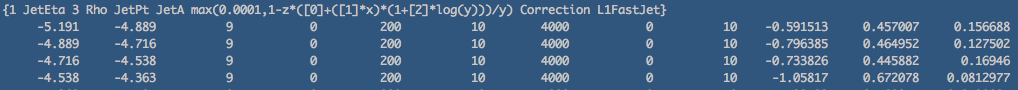
\includegraphics[width=\textwidth]{images/txtfile.png}
%			}
		\end{center}
%	\end{textblock}
	
	\begin{block}{How to read the JEC text files?}
		\begin{itemize}
		\item The \textbf{top row} establishes the definitions for the parameters to follow, the correction factor and the correction level being applied.
		\item The \textbf{first two columns} are the $\eta$ bins.
		\item The next column tells you how many numbers will follow it (in this case 9).
		\item The next number is the lower bound of the $\rho$, $p_{T}$ and jet area bins (the upper bound is the third number after that).
		\item Intsructions on how to apply the Jet Energy Corrections from a text file in FWLite environment. \\ 
		\footnotesize
		\href{https://twiki.cern.ch/twiki/bin/view/CMSPublic/WorkBookJetEnergyCorrections}{https://twiki.cern.ch/twiki/bin/view/CMSPublic/WorkBookJetEnergyCorrections}
		\end{itemize}
	\end{block}
}
%-----------------------------------------------------------------------------------------------------------
\frame{
\frametitle{What form do the corrections come in?}
\framesubtitle{Global Tag}
\begin{block}{Global Tag}
\begin{itemize}
\item Conditions data are defined in the Offline Conditions Database (ORCOF), which is read in CMSSW applications via Frontier caching servers.
\item The set of dataset tags which together define the offline conditions data are collected together in a \textbf{Global Tag (GT)}, which is itself stored in the database.
\item How to connect to a GT:
\end{itemize} 
\end{block}

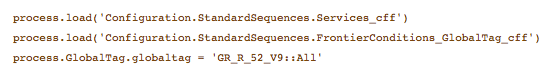
\includegraphics[width=10cm]{images/globaltag.png}

\begin{alertblock}{Note:}
\begin{itemize}
\item There can be many GT's for a given CMSSW release
\item It is important, therefore, that you know which conditions are in the GT you are using
\end{itemize}
\end{alertblock}

}
%-----------------------------------------------------------------------------------------------------------
\frame{
\frametitle{What form do the corrections come in?}
\framesubtitle{How to connect to a local sql file.}
\begin{columns}
\begin{column}{3.5cm}
\begin{block}{}
The recommended way of accessing JEC is with a global tag. The SQLlite file option is mainly used in the initial testing phase in preparation of a global tag.
\end{block}
\end{column}
\begin{column}{8.5cm}
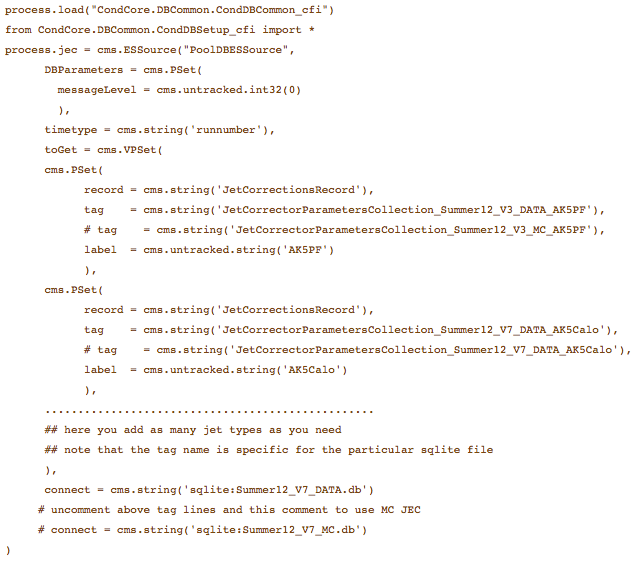
\includegraphics[width=8.5cm]{images/sqlfile.png}
\end{column}
\end{columns}

}
%-----------------------------------------------------------------------------------------------------------
\frame{
\frametitle{What form do the corrections come in?}
\framesubtitle{How to connect to a local sql file.}

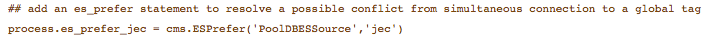
\includegraphics[width=11cm]{images/sql2.png}

\begin{block}{}
\begin{itemize}
\item When using a local SQL file, \textbf{es$\_$prefer} should be added to the process chain in the cfg file.
\item In this case, an \textbf{es$\_$prefer} indicates that whatever is defined in \textbf{es$\_$source} takes precedence over any other source for the condition object (in particular, the global tag).
\end{itemize}
\end{block}

}





